\subsubsection{Prijava za praktičnu obuku}

\vspace{3mm}

\begin{itemize}

\item \textbf{Kratak opis:} Da bi kandidat započeo praktičnu obuku potrebno je da se prijavi. Pre prijave kandidat dostavlja auto školi potvrde o obavljenom lekarskom pregledu, uplatama, nakon čega bira instruktora.

\vspace{2mm}

\item \textbf{Učesnici} \newline
   - Kandidat - korisnik sistema koji želi da se prijavi za praktičnu obuku.\newline 
   - Administrativni radnik - korisnik sistema koji proverava podatke, potvrđuje prijavu i šalje spisak instruktora.

\item \textbf{Preduslovi:} \newline
   - Sistem je u funkciji. \newline
   - Kadidat je položio teorijski ispit. \newline 
   - Kandidat je obavio lekarski pregled. 

\item \textbf{Postuslovi:} \newline
    - Kandidat se prijavio za praktičnu obuku 

\item \textbf{Osnovni tok:}  
   \begin{enumerate}
   \item Kandidat pristupa veb stranici i otvara formular za prijavu za praktičnu obuku.
   \item Sistem prikazuje formular.
   \item Kandidat popunjava formular.
   \item Kandidat klikom na dugme "Prijavi" šalje formular.
   \item Sistem evidentira prijavu.
   \item Sistem šalje podatke administrativnom radniku.
   \item Administrativni radnik proverava ispravnost i potpunost podataka.
   \item Administrativni radnik potvrdjuje prijavu i kandidatu šalje spisak slobodnih instruktora.
   \item Kandidat proverava mejl.
   \item Kandidat bira instruktora.
   \item Sistem belezi prijavu kandidata i izabranog instruktora.
   \end{enumerate}

\item \textbf{Alternativni tok:}  
   \begin{itemize}
   \item A1. \textbf{Neispravnost ili nepotpunost dokumentacije:}
  Ukoliko je u koraku 7 kandidat poslao nepotpun formular ili formular sadrži neke neispravne podatke, slučaj upotrebe se privremeno zaustavlja dok kandidat ne kompletira potrebnu dokumentaciju ili ispravi prosleđene podatke i proces se nastavlja od koraka 1 u osnovnom toku.
  \item A2. \textbf{Kandidat nije dobio mejl:}
  Ukoliko u koraku 9 kandidat nije dobio mejl o potvrdi prijave i spisak slobodnih instruktora, obaveštava administrativnog radnika i proces se nastavlja od koraka 8 u osnovnom toku.
   \end{itemize}

\end{itemize}  

\begin{figure}[H]
  \begin{center}
      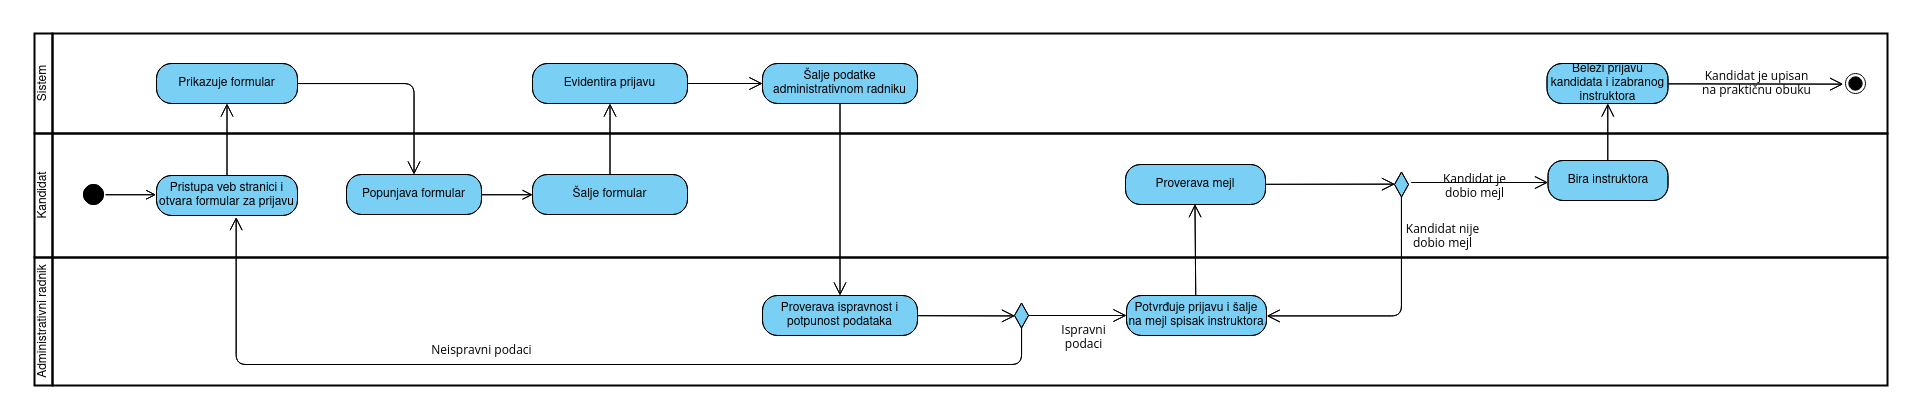
\includegraphics[width=140mm, height=70mm]{Diagrams/dijagram_aktivnosti_prijava_za_prakticnu_obuku.png}
  \end{center}
  \caption {Dijagram aktivnosti - Prijava za praktičnu obuku}
  \label{activity_prijava_za_prakticnu_obuku}

\end{figure}
